
\section{Simulation}\label{sec:simulation}

Two simulations were implemented using non-slip contact walls for position control.  The first controls the position of two robots, the second controls the position of $n$ robots.  

\subsection{Position Control of Two Robots}

Algorithm \ref{alg:optimalAlg}  was implemented in Mathematica using point robots (radius = $0$). 
%An online interactive demonstration and source code of the algorithm are available at \cite{Shahrokhi2015mathematicaParticle}.
  Fig.~\ref{fig:shapeControlMathematica1}  shows  an implementation of this algorithm with robot initial positions represented by hollow squares and final positions by circles. 
 Dashed lines show the shortest route if robots could be controlled independently, while solid lines show the optimal shortest  path using uniform inputs.
 
 The contour plots in Fig.~\ref{fig:contourPlots} top row show the length of the shortest path for given $s_1,s_2,g_1$ with $g_2$ ranging over all the workspace.  This plot clearly shows the nonlinear nature of the path planning, with multiple isolated islands showing regions that are difficult to reach. 
 If the length of each side of the square workspace is $L$, the worst case path length is $(\sqrt{2}+2)L$.
 
 The contour plots in Fig.~\ref{fig:contourPlots} bottom row show the same configurations, but plot the required number of moves.  There is never more than one $g_2$ position reachable in one move.  
 %If two-move solutions exist, they only appear along the boundary.
  If $g_2$ results in a contraction of $(\delta x, \delta y)$, there are many three move sequences. Four and five moves are sometimes required.






   %The path given by our algorithm is shown with solid arrows.
%Each row has five snapshots taken every quarter second. 
%For the sake of brevity axis-aligned moves were replaced with oblique moves that combine 
%jjkjk klklk klklklk klklk lklkl lklklklkl  klklklklk lklklklklk lklklkl klklklkl klklklk klklklk klklk klk klkl
% THES IMAGES DON'T DO THIS ANYMORE 
% $\Delta r_x$ is adjusted to $\Delta e_x$ in the second snapshot at $t = 0.25$. 
% The following frames  adjust $\Delta r_y$ to $\Delta e_y$. 
% $\Delta r_y$ is corrected by $t = 0.75$. 
% Finally, the algorithm moves the robots to their corresponding destinations.

\subsection{Position Control of $n$ Robots}
Alg. \ref{alg:PosControlNRobots}  was simulated in {\sc Matlab} using square block robots with unity width. %Code is available at \cite{Arun2015}.
 Simulation results are shown in Fig.~\ref{fig:4diagramsplots.pdf} for arrangements with an increasing number of robots,  $n$= [8, 46, 130, 390, 862]. 
The distance moved grows quadratically with the number of robots $n$. A best-fit line $210 n^2 + 1200n-10,000$ is overlaid by the data.

In Fig.~\ref{fig:4diagramsplots.pdf}, the amount of clearance is $\epsilon=1$.
Control performance is sensitive to the desired clearance.  As $\epsilon$ increases, the total distance decreases asymptotically, as shown in Fig.~\ref{fig:graphrobo.pdf}, because the robots have more room to maneuver and fewer $\operatorname{DriftMove}$s are required.
%We observed that the value of $\epsilon$, greatly affects the total number of moves of commanded moves on the robots. The smaller the value of �?� the greater is the number of moves required to move a said distance. The second graph plot(fig roboplot) is that of �?� vs �total commanded moves� which is the number of moves the global controller commands onto all the robots. Here we take the pattern 
%�ROBO� and calculate the �total commanded moves� for �?�=[ 0.25,0.375,0.5,0.625,0.75,0.875,1]. We can notice an exponential fall in the total command moves. It can be inferred that there is a tradeoff between area of bounded region and the number of moves. For smaller �?�, smaller is the required area to implement algorithm but the longer is the time taken to complete the algorithm. Fig robo
%Unit of �?� is the ratio of minimum clearance value to the body length of a robot.




\begin{figure}
\begin{center}
	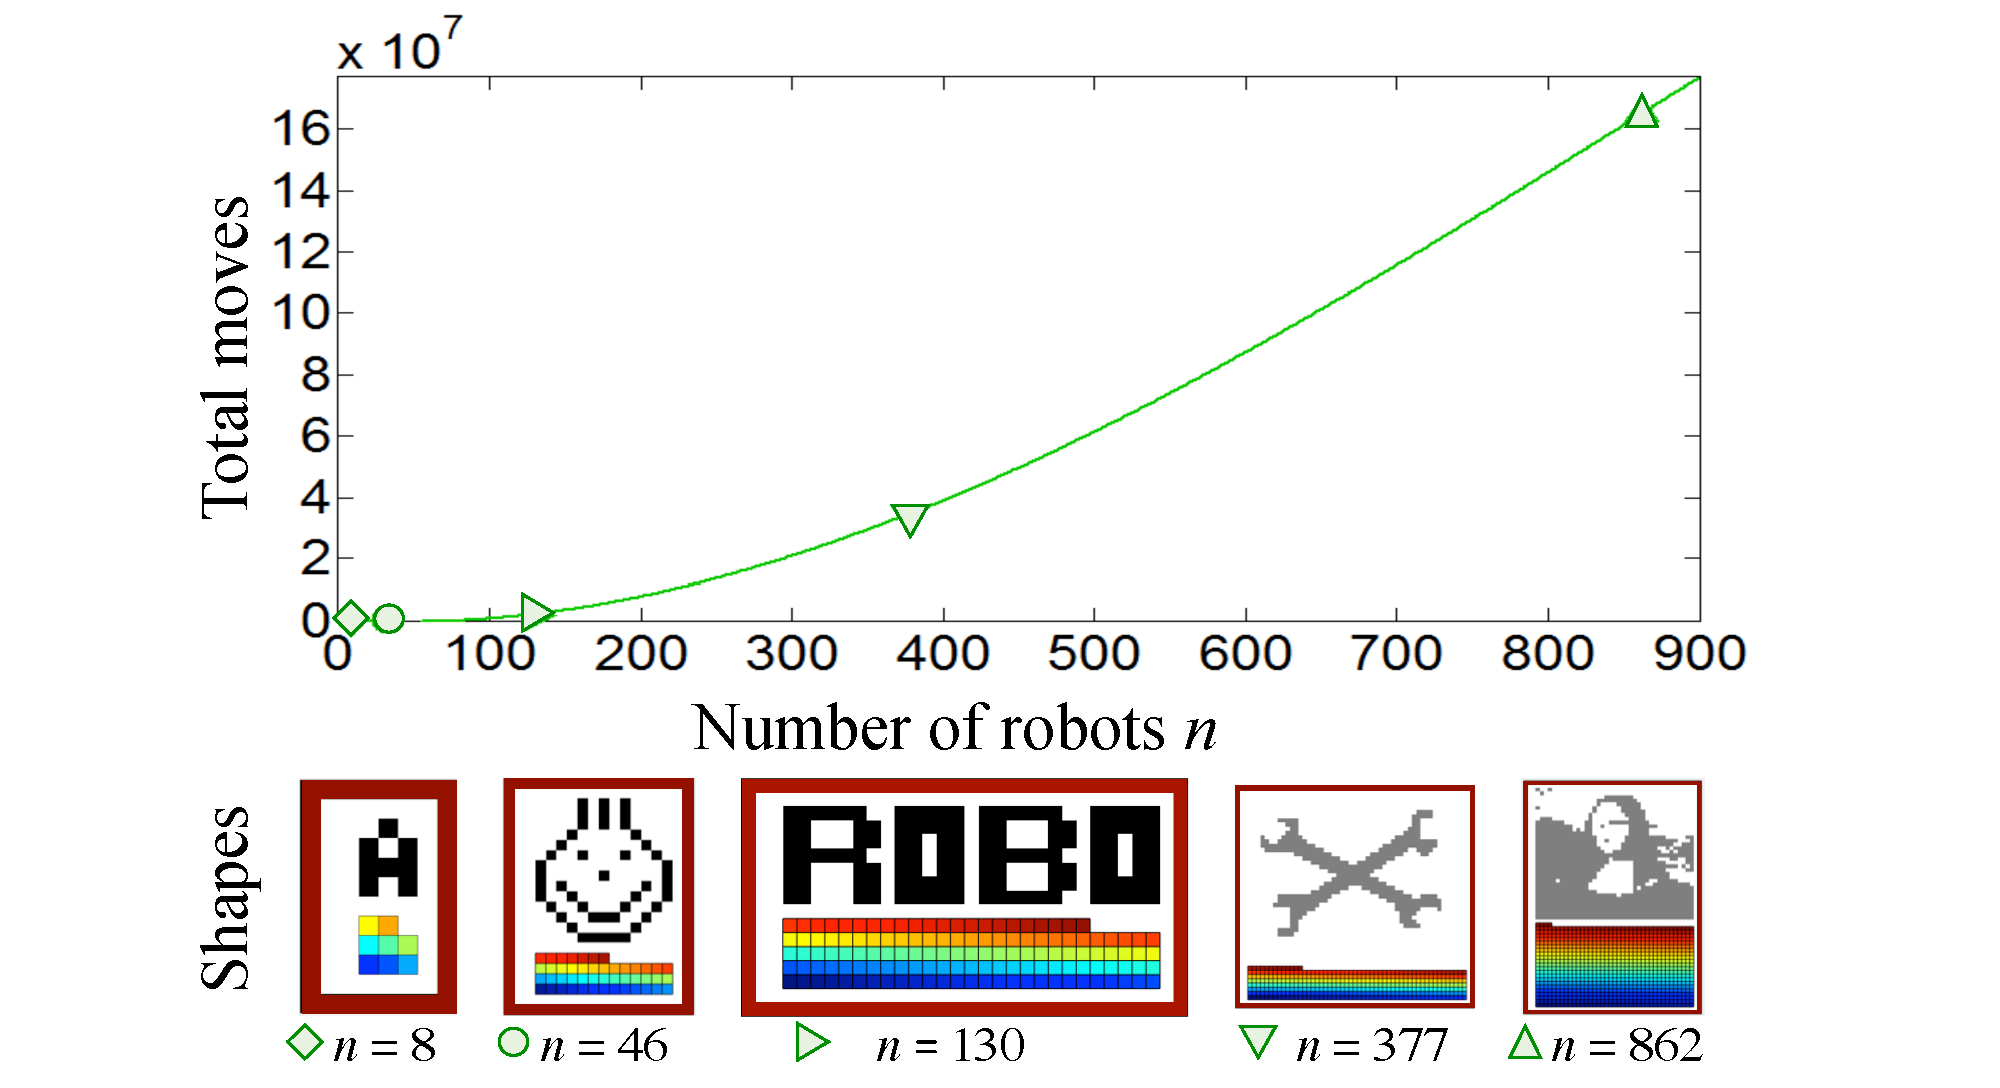
\includegraphics[width=\columnwidth]{5diagramsplots2.pdf}
\end{center}
\vspace{-1em}
\caption{\label{fig:4diagramsplots.pdf}
The required number of moves under Alg.~\ref{alg:PosControlNRobots} using non-slip contact walls to rearrange $n$ square-shaped robots grows quadratically with $n$. % \cite{Arun2015}.
 See code at \cite{Arun2015}.
}
\end{figure}

\begin{figure}
\begin{center}
	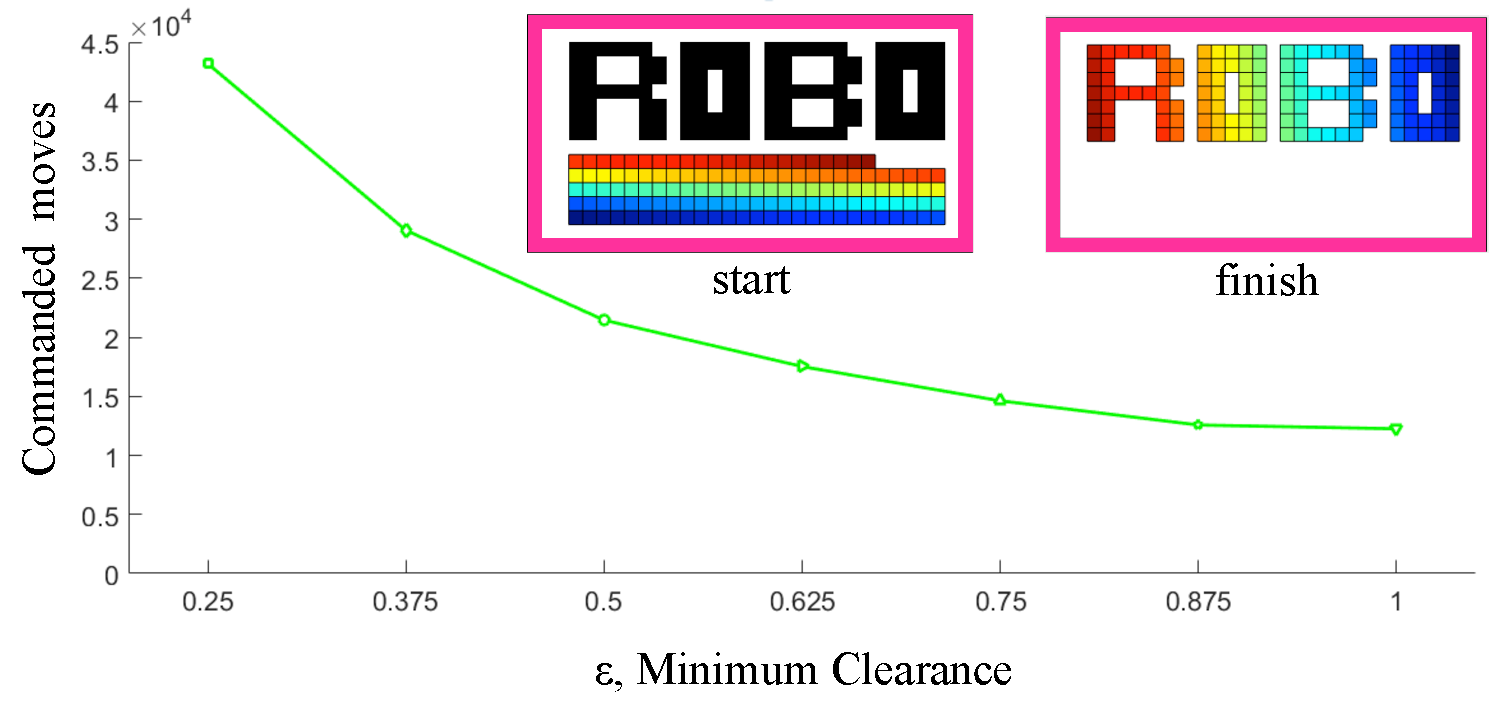
\includegraphics[width=\columnwidth]{graphrobo.pdf}
\end{center}
\vspace{-1em}
\caption{\label{fig:graphrobo.pdf}
Control performance is sensitive to the desired clearance $\epsilon$.  As $\epsilon$ increases, the total distance decreases asymptotically.
}\vspace{-1em}
\end{figure}


